\documentclass[a4paper,10pt,titlepage,bibliography=totocnumbered]{scrartcl}
\usepackage[utf8]{inputenc}
\usepackage{times}
\usepackage[english]{babel}
\usepackage{amsmath}
\usepackage{amsfonts}
\usepackage{amssymb}
\usepackage{fancyref}
\usepackage{graphicx}
\usepackage{listings}
\usepackage{pdfpages} 
\usepackage{listings}
\usepackage{color}
\usepackage{caption}
\usepackage{subcaption}
\usepackage[lmargin=2cm,rmargin=2cm,tmargin=2cm,bmargin=2cm]{geometry}


\lstset{
    frameround=fttt,
    language=Java,
    breaklines=true,
    keywordstyle=\color{blue}\bfseries, 
    basicstyle=\ttfamily\color{blue},
    numberstyle=\color{black}
    }
\lstMakeShortInline[columns=fixed]|

\inputencoding{utf8}
\parindent0em

%\usepackage{fancyhdr}
%\pagestyle{fancy}

%opening
%\fancyhf{}
%Titel der Veranstaltung -- Ersetze X durch Zettelnr.
%\fancyhead[L]{\textbf{}}
%%Dein Name
%\fancyhead[C]{\textbf{}}
%%Dein Tutor
%\fancyhead[R]{\textbf{}}
%\fancyfoot[C]{\thepage}

\subject{Conversation Animation for Virtual Humans}
\author{Vanessa da Silva, Yannick Bröker}
\title{IdleBehaviour with AsapRealizer}
\subtitle{An implementation with Motion Graphs}
\date{17. August 2015}


\newcommand{\slerp}{\mathrm{slerp}}

\newcommand*{\titleGM}{\begingroup % Create the command for including the title page in the document
\hbox{ % Horizontal box
\hspace*{0.2\textwidth} % Whitespace to the left of the title page
\rule{1pt}{\textheight} % Vertical line
\hspace*{0.05\textwidth} % Whitespace between the vertical line and title page text
\parbox[b]{0.75\textwidth}{ % Paragraph box which restricts text to less than the width of the page

{\noindent\Huge\bfseries IdleBehaviour with AsapRealizer \\[0.5\baselineskip]  \huge \textcolor{gray}{An implementation with Motion Graphs}}\\[2\baselineskip] % Title
{\large \textit{Conversation Animation for Virtual Humans}}\\[4\baselineskip] % Tagline or further description
{\Large \textsc{Vanessa da Silva, Yannick Bröker}} % Author name

\vspace{0.5\textheight} % Whitespace between the title block and the publisher

}}
\endgroup}




\begin{document}

\begin{titlepage}
\titleGM
\end{titlepage}

\tableofcontents

\newpage

\section{How To Run}

\subsection{gesturebinding}

In the gesturebindung, the RestPose needs to be specified:

\begin{lstlisting}[language=XML]
<RestPoseSpec>
    <constraints>
        <constraint name="stance" value="STANDING"/>
        <constraint name="BODY" value="IDLE"/>
    </constraints>
    <RestPose type="class" class="asap.realizerdemo.idle.IdleMovement"/>
</RestPoseSpec>
\end{lstlisting}


\subsection{BML}

After loading the gesturebinding in the animation-engine-configuration, the Idle-Movement can be started with the following BML:

\begin{lstlisting}[language=XML]
<bml id="bml1" xmlns="http://www.bml-initiative.org/bml/bml-1.0">
    <postureShift id="pose1" start="0">
        <stance type="STANDING"/>
        <pose part="BODY" lexeme="IDLE"/>
    </postureShift>
</bml>
\end{lstlisting}
\clearpage
\section{Used Techniques}

\subsection{MotionGraphs}
\label{sec:motiongraph}
We initialize the MotionGraph with a List of captured motions, given as SkeletonInterpolators, where nodes represent the start and end of a motion while the edges represent the motion itself.(cf. \fref{fig:at_start}.)

\begin{figure}[ht]
\centering
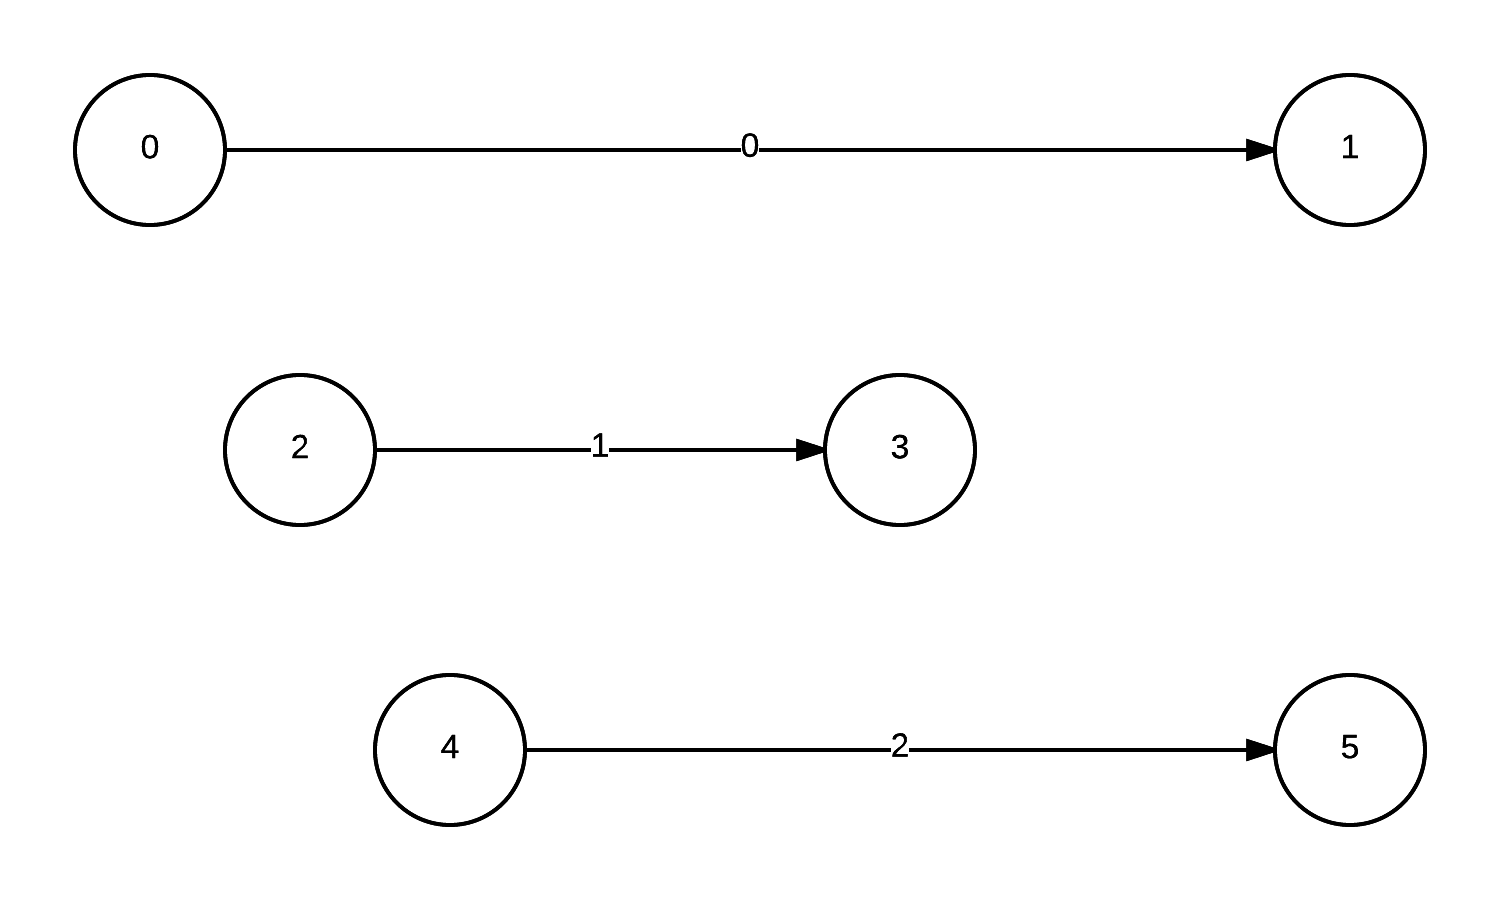
\includegraphics[width=\textwidth/2]{img/1_GraphAtStart.png}
\caption{initial Graph}
\label{fig:at_start}
\end{figure}

When trying to add mirrored motions, we discovered an error in \lstinline{SkeletonInterpolator.mirror()}, so we made it optional. It can be triggered with \lstinline{MotionGraph.MIRRORED}. If you only want the mirrored motions, you can disable the normal motions with \lstinline{MotionGraph.NORMAL}.\\


After loading the graph we split the existing motions to gain more nodes in the graph. Currently, we just split motions in equally long pieces. A better way could be to detect frames without any movement and cut them there.
\\
\fref{fig:after_split} displays the graph after splitting.

\begin{figure}[ht]
\centering
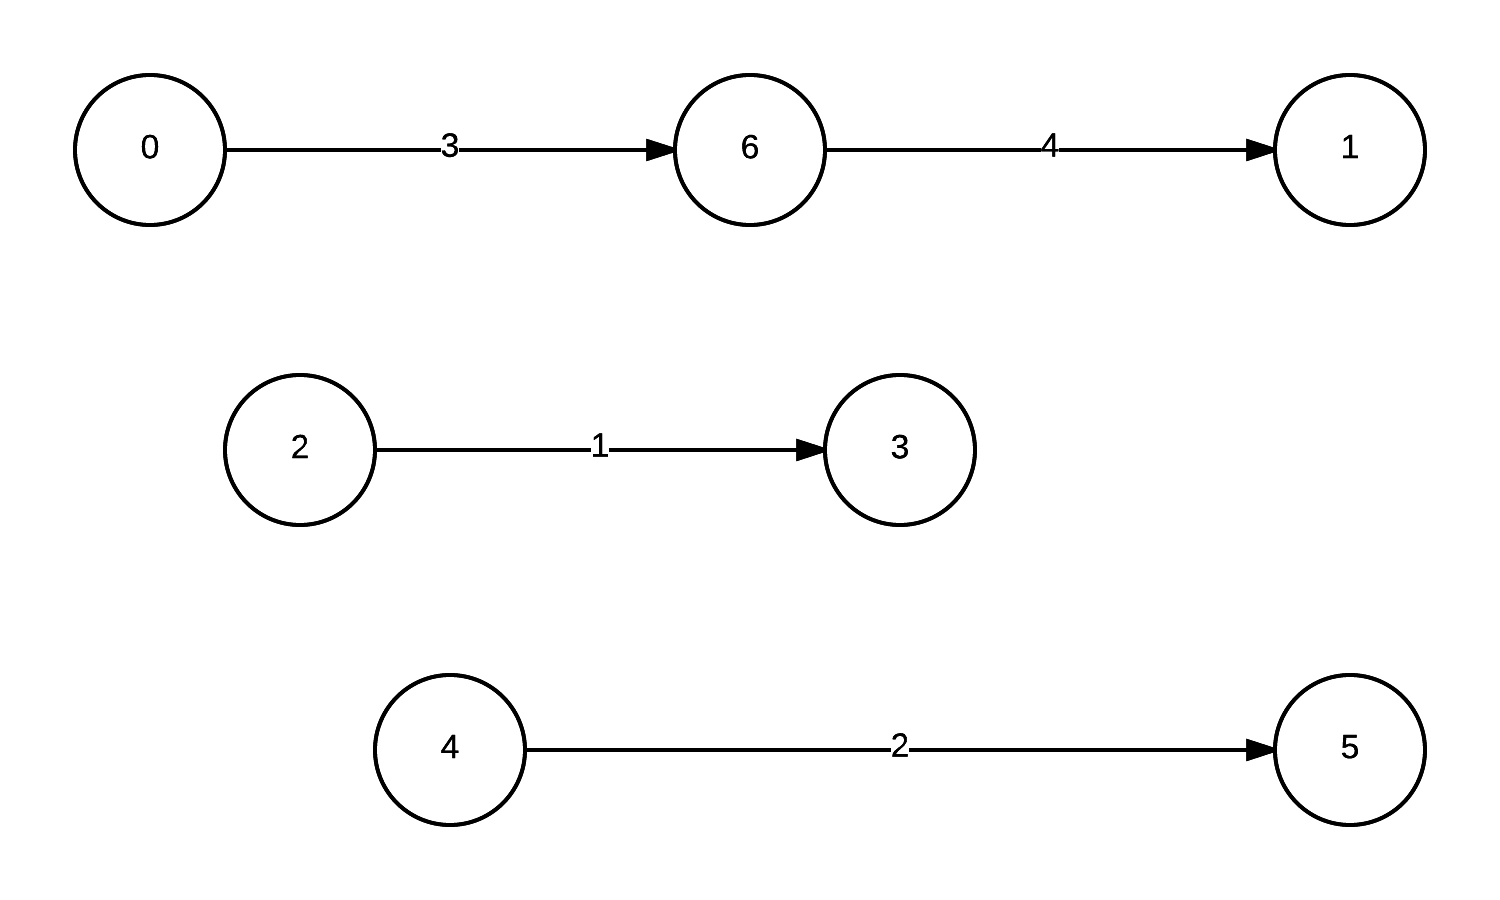
\includegraphics[width=\textwidth/2]{img/2_GraphAfterSplit.png}
\caption{Graph after splitting}
\label{fig:after_split}
\end{figure}


After splitting, we use a Distance Metric (as described in \fref{sec:distanceMetric}) to find motions, that are equal enough for blending.
\\
To blend two motions, we cut both of them into two pieces, where the end-piece of the first and the start-piece of the second motion are the parts used for blending. In this process two new nodes are created which mark the cuts.The blended motion - created like described in \fref{sec:blending} - then connects those new nodes.
\\\\
Currently, we compare and blend 100 frames per motion. We tried multiple values, but they didn't lead to better results in general, so we remain at 100 frames.
\\
It may be better to change the number of blended frames based on the distance, but that would have exceeded this projects scope.\\
It may become an option when dealing with our Bachelor Thesis. 
\newpage In \fref{fig:first_blend}, motion 3 shall be blended with motion 1. Therefore both are cut into pieces to create new nodes to mark the beginning and the end of the blended motion. (cf. \fref{fig:cut}). Then, motion 6 and motion 7 are blended to create motion 9, which now connects motion 5 and 8.
\\
The connected motions 5,9 and 8 are now a smooth transition from node 0 to 3. (cf. \fref{fig:blended})


\begin{figure}[h]
\centering
\begin{subfigure}[b]{0.4\textwidth}
	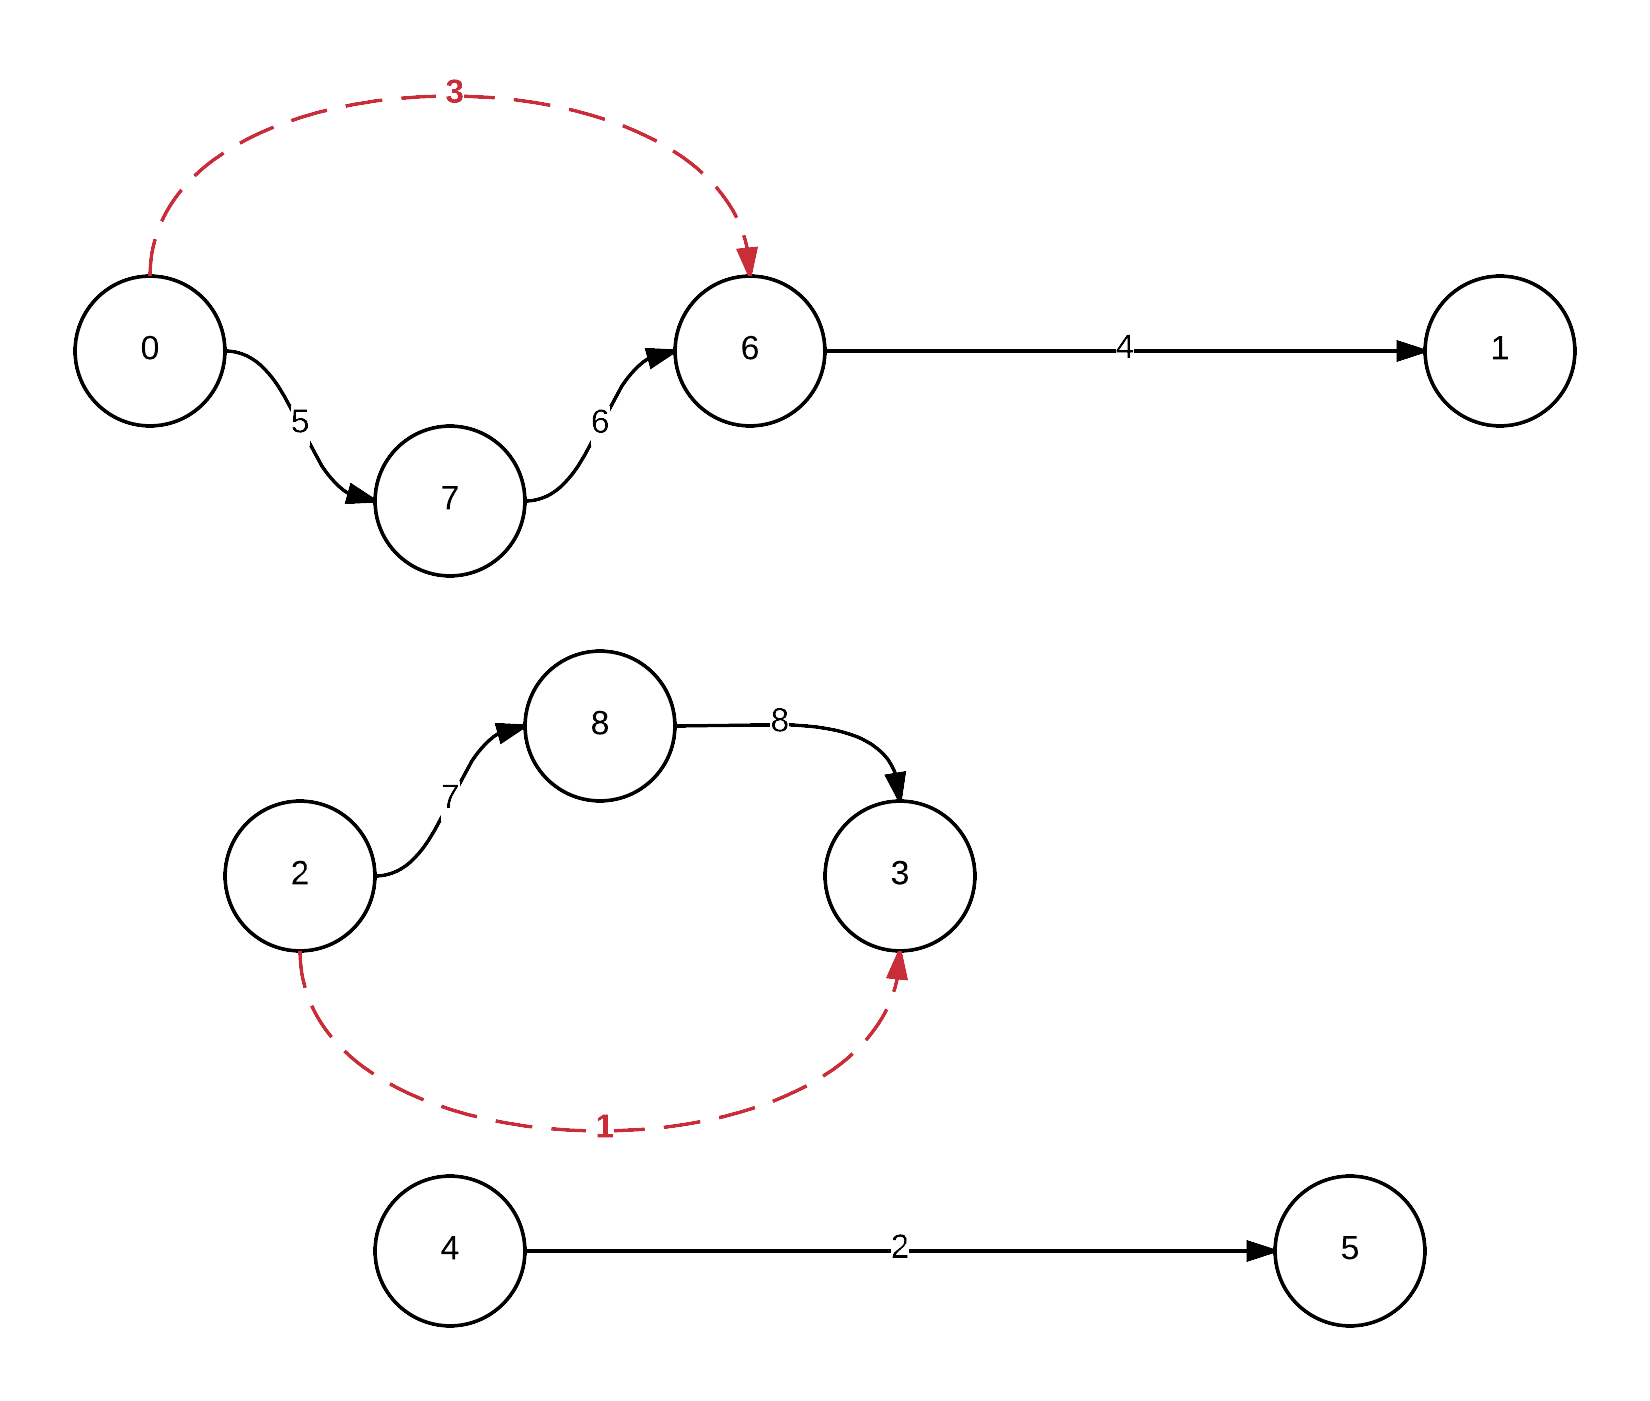
\includegraphics[width=\textwidth]{img/3a_GraphAfterCut.png}
        \caption{Graph after cutting for blends }
        \label{fig:cut}
\end{subfigure}
\begin{subfigure}[b]{0.4\textwidth}
	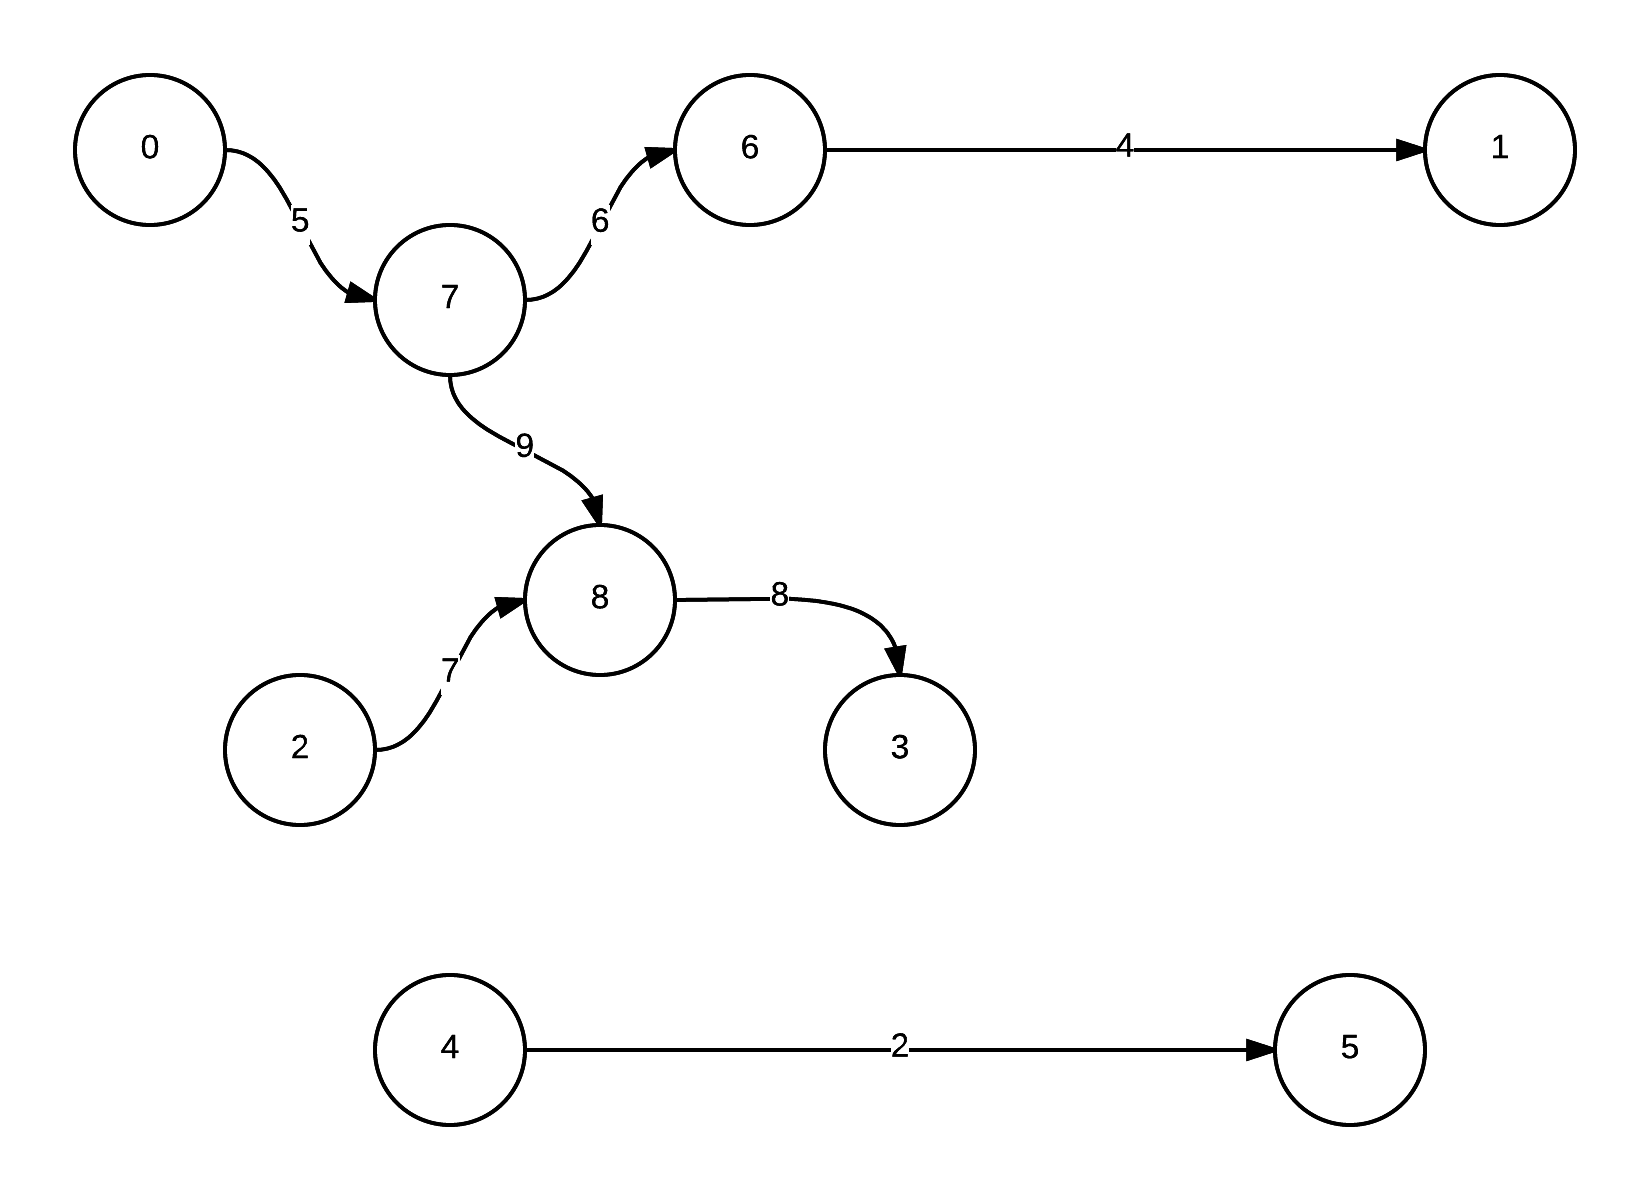
\includegraphics[width=\textwidth]{img/3b_GraphAfterBlend_0+1.png}
	\caption{Graph after blending}
\label{fig:blended}
\end{subfigure}
\caption{Process of blending}
\label{fig:first_blend}
\end{figure}


\fref{fig:fullyBlended} shows an exemplary Motion Graph, after all possible blendings have been created.
\\
It already contains endless motions, which are concatenations of single motions, but also Dead-Ends - nodes that don't have any successors.
Reaching one of these during a random-walk would bring the motion to an end. Therefore such dead-ends have to be removed from the graph.


\begin{figure}[h]
\centering
\begin{subfigure}[b]{0.4\textwidth}
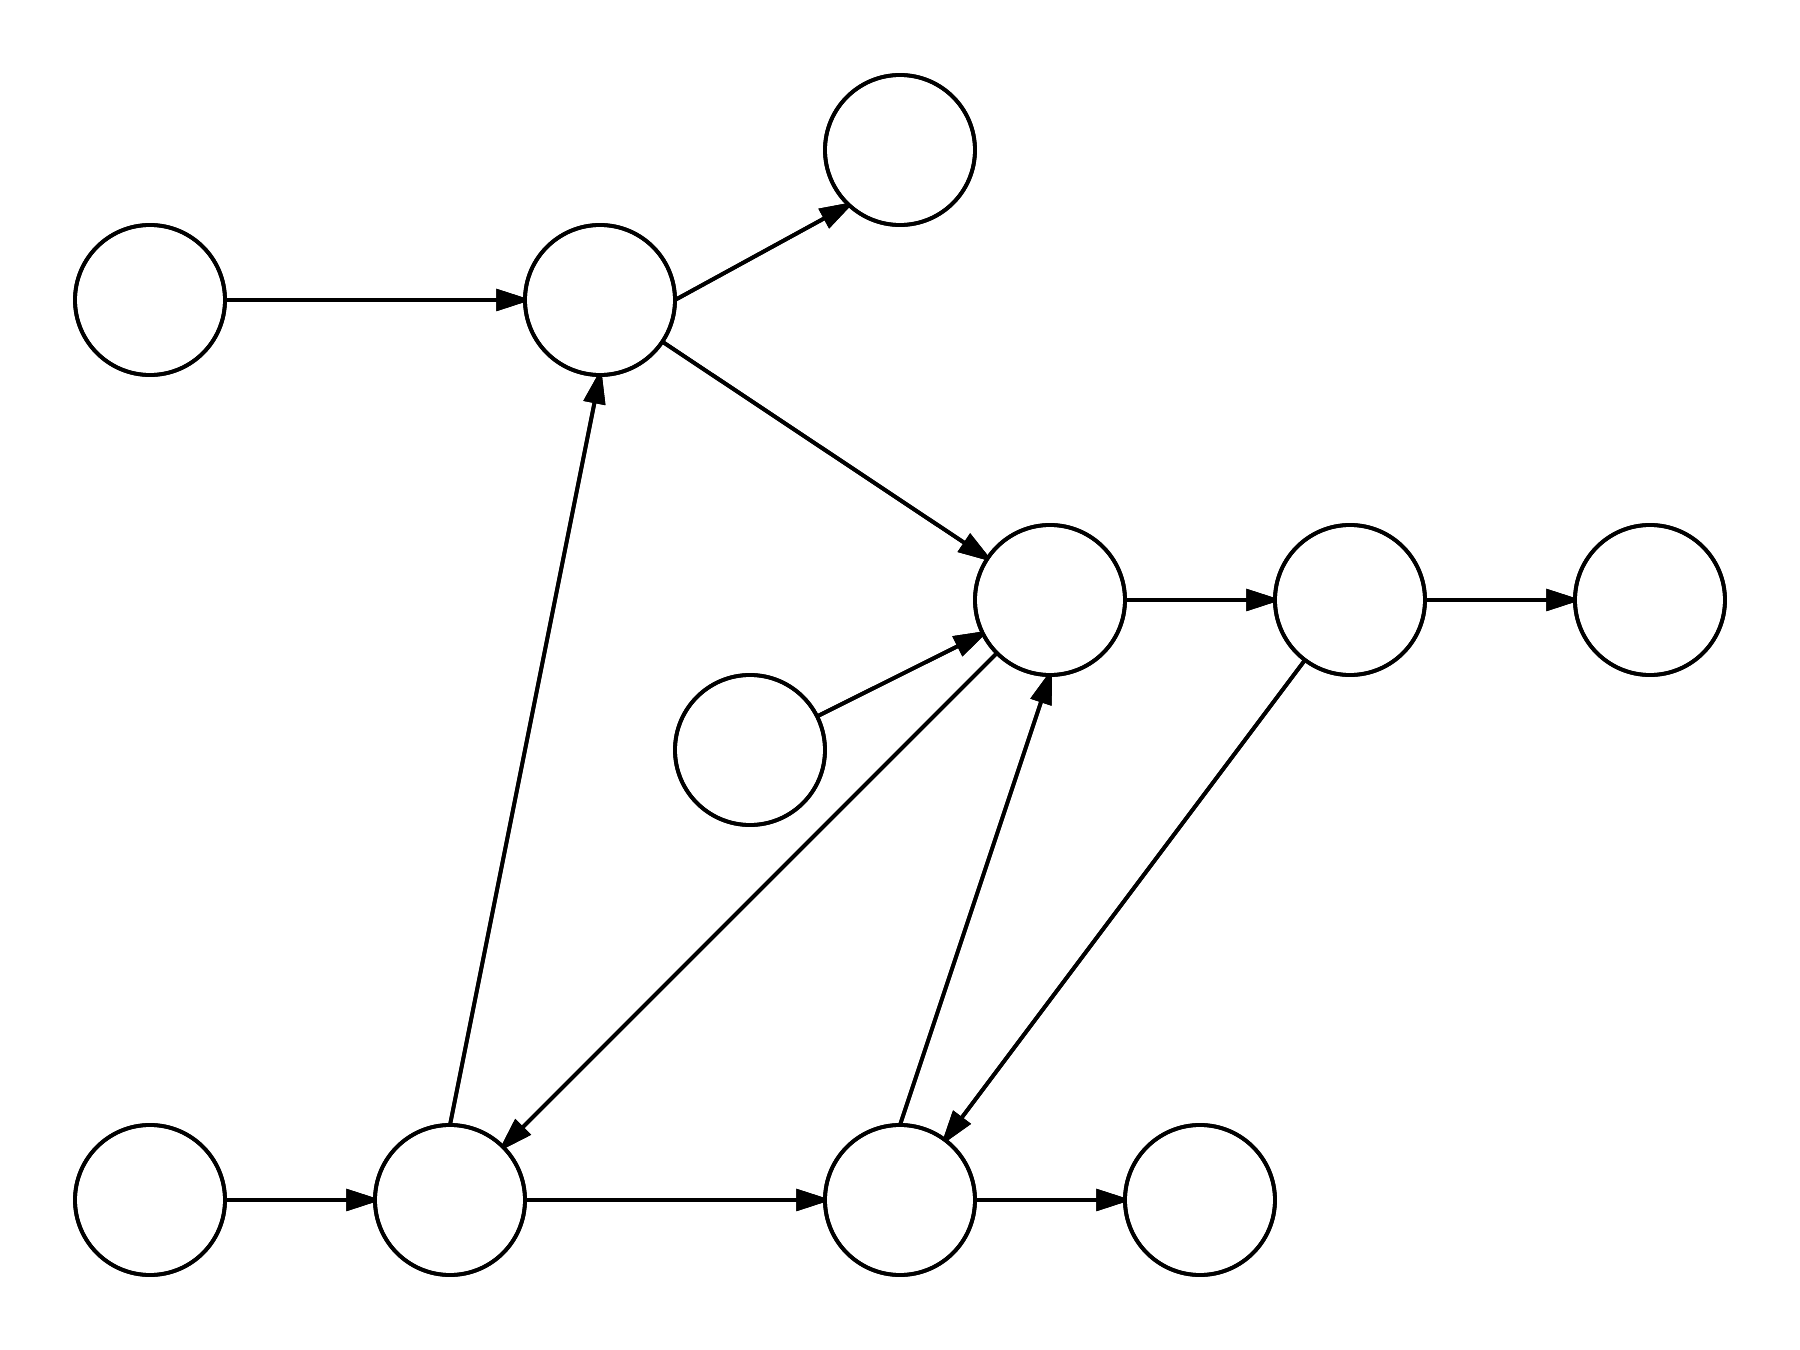
\includegraphics[width=\textwidth]{img/4_GraphAfterAllBlends.png}
	\caption{Graph after blending}
        \label{fig:fullyBlended}
\end{subfigure}
\begin{subfigure}[b]{0.4\textwidth}
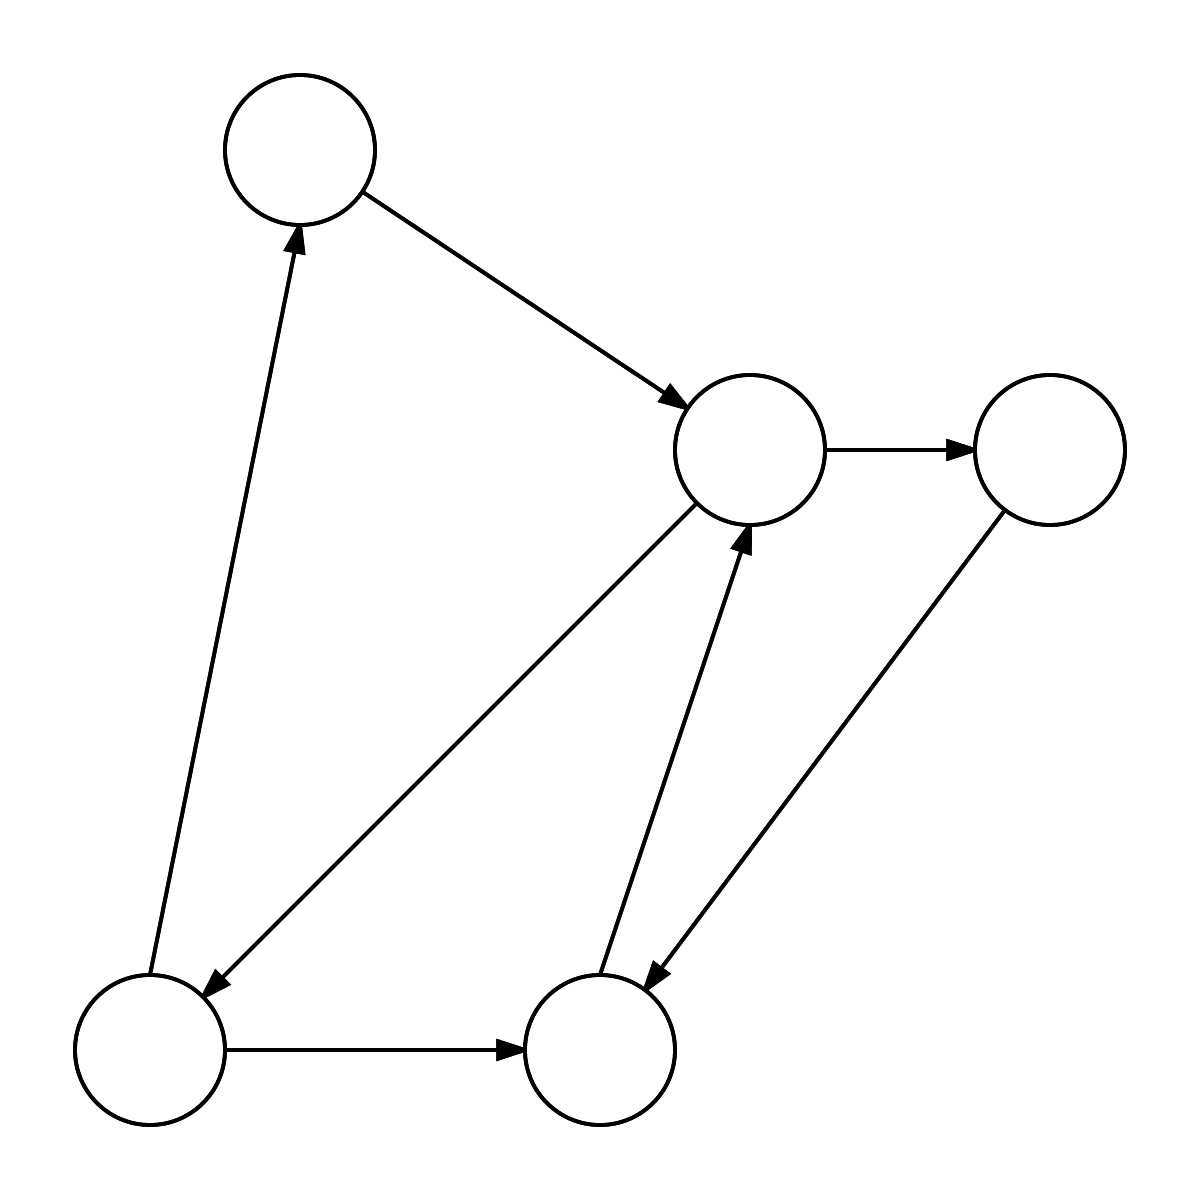
\includegraphics[width=\textwidth]{img/5_GraphAfterPruning.png}
\caption{Graph after pruning}
\label{fig:pruned}
\end{subfigure}
\caption{Pruning}
\end{figure}


After pruning, there is at least one following motion for every node in the graph. This guarantees an endless random-walk. (cf. \fref{fig:pruned})



\subsection{Distance Metrics}
\label{sec:distanceMetric}

As default Distance-Metric we use a Joint-Angles-Metric based on the one described in \cite[4.1 Joint angles]{vanbasten2009}.
Because velocity isn't very relevant in idle-motions, we only compare root-positions and joint-angles.

\begin{align}
d(a,b) = (p_a-p_b)^2 + \sum_{k \in J} w_{k} (\log(q_{a,k}) - \log(q_{b,k}))^2
\end{align}

Also, the weights we use are different than described in the paper. 

Since legs seldom move very much during idle movement, but their absolute position may vary between different motions, blending can result in the feet sliding over the floor. This is unnatural-looking behavior. 

Other limbs, like hands and arms can be blended from every position, without looking unnatural.

Based on this, we chose the weights for hips, knees and ankles very high, and all other weights low.
\\\\
If the Distance is lower than 20, (see \lstinline{MotionGraph.DEFAULT_THRESHOLD}), the Motions are 'close' enough to be blended. We experimented with different thresholds, but decided to stick to this one. 
\\
Because the threshold is strongly connected to the weights, only one of those values has to be changed, whenever different results shall be achieved. \\
In later versions, it may be better to change the threshold to 1 and set the weights accordingly, for better understanding or using other metrics.
\\
See  \fref{sec:jointangles} for more information on the current metric.


\subsection{Blending}
\label{sec:blending}

We use the simple blending as described in \cite[3.3 Creating Transitions]{kovar2012} instead of the one described in \cite{kovar2003}.
\\
The second one may lead to better results, but is much more complicated while the first one already serves it's purpose. Blending with registration curves as in \cite{kovar2003} is more useful with Motion Graphs that contain much movement, like walking, jumping etc, which is not the case in idle-movement. Maybe, it can be implemented in a later version to see differences between the two blending-techniques.
\\\\
The blending is calculated as follows:

The root-position is just a linear transition between the two original positions:
\begin{align}
\label{root_blend}
p_i=\alpha * p_{a_i} + 1-\alpha * p_{b_i}
\end{align}

Where \(p_a \)and \(p_b\) are the root-positions of the blended frames, \(i\) ist the index of the blended frame, and \(p\) is the resulting position.
\\\\
The rotation of each joint is calculated with the slerp-algorithm:

\begin{align}
\label{rot_blend}
r_{j_i} = \slerp(r_{a_{j_i}},r_{b_{j_i}}, 1-\alpha)
\end{align}

Where \(r_{a_{j_i}}\) and \(r_{a_{j_i}}\) are the rotations of joint \(j\) at frame \(i\), and \(r_{j_i}\) ist the resulting rotation.
\\
(We need to use \(1-\alpha\) in \(\slerp\), some other implementations (e.g. the papers) use \(\alpha\).)
\\\\
\(\alpha\) ist calculated with the following formula, which results in better motions than just a linear transition from 0 to 1.

\begin{align}
\alpha = 2 * \left( \frac{i+1}{k} \right)^3 - 3 * \left( \frac{i+1}{k} \right)^2 + 1
\end{align}

Where \(i\) is the frames index as in \eqref{root_blend} and \eqref{rot_blend}, and \(k\) ist the number of frames that are to be blended.


\subsection{Alignment}
\label{sec:alignment}

Before calculating the distance between motions and blending them, they need to be aligned.
\\
Not all motions have the same root-position and rotation, so unaligned blending would result in unnatural sliding, for the blended root would slide between the two original ones.
\\
To avoid this, we bring the root-positions of the first frame of both motions in line with each other. We then rotate the model around the Y-axis, so both frames 'look' into the same direction. Rotation around X and Z doesn't need to be aligned, because these are part of the motion.

\section{Extensibility}

\subsection{Loading mocap files}

Currently, other motion-capture-files could only be defined in IdleMovement.java. Sadly, after this, the whole package needs to be recompiled, so we hope theres a better way in a later Version of AsapRealizer.\\
In the version of AsapRealizer we use, the only way to set different files without recompiling are the parameters in the BML, but those parameters are set while running the RestPose, so the MotionGraph would be calculated when the RestPose is started, which leads to a delay of a few seconds.

\subsection{Other Classes for Blending etc.}

The Motion Graph is constructed to be used with other classes for metrics, e.g. PointCloudMetric as described in \cite{vanbasten2009}, different Alignment etc.
We use a Builder (\lstinline{MotionGraph.Builder}) to set those classes and create an instance of the graph.
\\\\
Setting different classes is only possible in IdleMovement.java, which results to the same problems as loading other mocap files.


\section{System overview}

\subsection{IdleMovement}

The RestPose, which can be started with BML.

It uses the MotionGraph to generate real-looking, infinite Motions for idle-behavior.
\\\\
If it's started, it gets the motion which should be played with \lstinline[]{MotionGraph.next()}, and aligns position, rotation and time
\\\\
Currently, if the idle-behaviour ist running, it overrides every other behaviour that may be started afterwards. This could be fixed in a later version, maybe a Bachelor Thesis.

\subsection{IMotionGraph}

Interface for Motion Graphs.
Its only Method is \lstinline[]{next()}, which returns a following Motion (as SkeletonInterpolator) in the MotionGraph.

\subsection{MotionGraph}

Our MotionGraph-Implementation.
\\
It's described in \fref{sec:motiongraph}.

\subsection{MotionGraphBuilder}

Our Builder for the MotionGraph. It's implemented to easily construct a MotionGraph with different implementations for each aspect.
\\
It's not necessary, but was usefull for changing different Parts of the MotionGraph.

\subsection{IDistance}

Interface for DistanceMetrics.

\subsection{JointAngles}
\label{sec:jointangles}
Our implementation of a DistanceMetric. It's based on the Joint-Angle-Method as described in \cite[4.1 Joint angles]{vanbasten2009} with few changes.
We only compare root-positions and joint angles, and ignore the velocities. Thats mainly because joint velocities are very low in idle motions and if they are also low-weighted, they tend to be close to 0.
\\\\
The weights we use are stored in WeightMap, which is an implementation of a map. It holds weights for each joint, and ignores the L\_- and R\_-prefixes of joint-names.
\\
See \fref{sec:distanceMetric} for more information.

\subsection{IBlend}

Interface for Blendings

\subsection{Blend}

Our Implementation of a blending, as described in \cite[3.3 Creating Transitions]{kovar2012}, see  \fref{sec:blending} for an explanation.

\subsection{IAlignment}

Interface for Alignment.

\subsection{Alignment}

Our implementation of an alignment, see \fref{sec:alignment} for an explanation.

\subsection{NopAlignment}

It's an implementation that doesn't align anything at all, but was usefull for testing.

\subsection{ISplit}

Interface for Splitting.
\\\\
We think, a good implementation could split long, captured motions, that contain different unrelated motions, into pieces, which contain only one motion.

\subsection{DefaultSplit}

Our Implementation currently splits Motions in pieces with lenght around 2.5 seconds.


\bibliographystyle{abstract} \bibliography{report}

\end{document}